\documentclass[10pt]{article}

% Lines beginning with the percent sign are comments
% This file has been commented to help you understand more about LaTeX

% DO NOT EDIT THE LINES BETWEEN THE TWO LONG HORIZONTAL LINES

%---------------------------------------------------------------------------------------------------------

% Packages add extra functionality.
\usepackage{times,graphicx,epstopdf,fancyhdr,amsfonts,amsthm,amsmath,algorithm,algorithmic,xspace,hyperref}
\usepackage[left=1in,top=1in,right=1in,bottom=1in]{geometry}
\usepackage{sect sty}	%For centering section headings
\usepackage{enumerate}	%Allows more labeling options for enumerate environments 
\usepackage{epsfig}
\usepackage[space]{grffile}
\usepackage{booktabs}
\usepackage{forest}
\usepackage{enumitem}   
\usepackage{fancyvrb}
\usepackage{todonotes}
\usepackage{setspace}


% This will set LaTeX to look for figures in the same directory as the .tex file
\graphicspath{.} % The dot means current directory.

\pagestyle{fancy}

\lhead{Final Project}
\rhead{\today}
\lfoot{CSCI 334: Principles of Programming Languages}
\cfoot{\thepage}
\rfoot{Spring 2024}

% Some commands for changing header and footer format
\renewcommand{\headrulewidth}{0.4pt}
\renewcommand{\headwidth}{\textwidth}
\renewcommand{\footrulewidth}{0.4pt}

% These let you use common environments
\newtheorem{claim}{Claim}
\newtheorem{definition}{Definition}
\newtheorem{theorem}{Theorem}
\newtheorem{lemma}{Lemma}
\newtheorem{observation}{Observation}
\newtheorem{question}{Question}

\setlength{\parindent}{0cm}

%---------------------------------------------------------------------------------------------------------

% DON'T CHANGE ANYTHING ABOVE HERE

% Edit below as instructed

\title{Twined Language Specification} % Replace SnappyLanguageName with your project's name

\author{Lucas Weissman \and Zach Sturdevant} % Replace these with real partner names.

\begin{document}
  
\maketitle

\subsection*{Introduction}

"Twined" represents a transformative approach in how we manage and interact
 with textual information. By converting unstructured text data from diverse 
 note-taking formats into structured, navigable knowledge graphs, "Twined" 
 provides a unique visual perspective that enhances comprehension and analysis.
 \singlespacing


 Rules:
 Graph Rule: {x, y}, {x, z} → {x, z}, {x, w}, {y, w}, {z, w}
 \singlespacing
 Hypergraph Rule: {x, y, z} → {x, u, v}, {z, v, w}, {y, w, u}
 \singlespacing


 graph: {Sunlight,Plant Growth},{Water,Plant Growth},{Soil Nutrients,Plant Growth}
 \singlespacing
 hypergraph: {Sunlight,Water,Soil Nutrients,Plant Growth},{Temperature,Humidity,Water,Plant Growth}
 \singlespacing


\singlespacing
\todo[inline]{Delete this TODO and replace with 2+ paragraphs.}
\singlespacing

Brainstorming Section:

“Twined” intertwines user’s information by managing and interacting with textual 
information. It converts unstructured text data from various note-taking formats 
into structured, navigable knowledge graphs. This will allow users to quickly 
visualize connections and gain insights that might be missed in traditional 
textual data formats. 

\singlespacing
A hypergraph is defined as a collection of nodes and hyperedges, where each 
hyperedge has the capability to connect three or more nodes, unlike traditional
graphs where edges connect only two nodes. In terms of mathematical 
representation, edges in standard graphs are noted as pairs of numbers within 
curly brackets, such as {1, 2}. Conversely, in hypergraphs, hyperedges 
that connect multiple nodes are denoted by three or more numbers within 
curly brackets, for example, {1, 2, 3}. Visually, in graphs, edges are depicted
as connections between white dots (nodes) using white arrows (edges). 
Hypergraphs extend this visualization by linking three or more white dots 
(nodes) with multiple arrows and a transparent white web, highlighting the
complex relationships between nodes.

\singlespacing
PS. We might adjust the intro to fit within the context of our current 
deliverables, or we could state the end goal briefily and current stage 
we are in with the test cases we have built. - Lucas

\newpage
\subsection*{Design Principles}

\singlespacing
\todo[inline]{Delete this TODO and replace with 1+ paragraphs.}
\singlespacing

Brainstorming Section:


\newpage
\subsection*{Examples}



\begin{figure}[!hb]
    \centering
    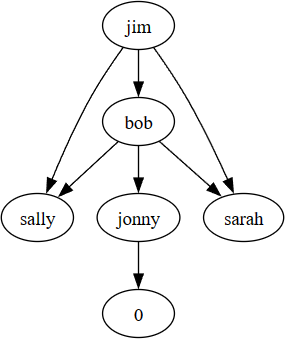
\includegraphics[width=0.3\linewidth]{images/family_test_0.1.png} 
    \caption{Family Relationship}
    \label{figure 1:}
\end{figure}

This graph represents the relationships between family individuals. Each node represents 
a person, and each edge represents a direct relationship between two individuals. For example,
"bob" has relationships with "sally," "jonny," and "sarah," as depicted by the edges 
connecting their respective nodes. 

\begin{figure}[!hb]
    \centering
    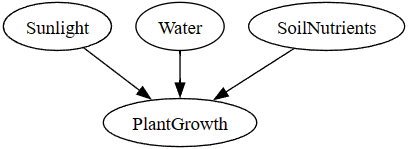
\includegraphics[width=0.4\linewidth]{images/plant_test_0.1.png} 
    \caption{Plant Growth Relationship}
    \label{figure 2:}
\end{figure}

The graph represents factors affecting plant growth. Each node represents
a factor such as "Sunlight," "Water," and "Soil Nutrients," and each edge 
represents the influence of these factors on "Plant Growth," as depicted 
by the edges connecting their respective nodes.


\singlespacing
\todo[inline]{Delete this TODO and replace with 3+ examples and accompanying descriptions.}
Brainstorming Section
\singlespacing

I have added above an example of image insertion from one of our test cases, we could replace 
it with a few more/new ones. - Lucas

\newpage
\subsection*{Language Concepts}

The language concepts behind "Twined" incorporate elements from graph theory 
and data visualization to support the creation of knowledge graphs and 
hypergraphs. These concepts are integral in defining how textual data is parsed, 
how entities within the text are identified as nodes, and how relationships (edges)
are established based on the context and content of the data. This allows "Twined"
to dynamically interpret and display information in a way that highlights
both hierarchical and associative relationships.



\singlespacing
\todo[inline]{Delete this TODO and replace with 1+ paragraphs.}
\singlespacing

Brainstorming Section

Terms to be used/contextualized:
Graph Theory
Data Visualization
Knowledge Graphs
Hypergraphs
Parsing
Nodes
Edges
Hierarchical Relationships
Associative relationships

\newpage
\subsection*{Formal Syntax}
\singlespacing

\begin{tabular}{lll}
    $<\textbf{expression}>$ & ::= & $<\textbf{Node}>$  \\
                            & $|$  & $<\textbf{edgeList}>$ \\
                            & $|$  & $<\textbf{nodeName}>$ \\
                            & $|$  & $<\textbf{listOfNodes}>$ \\
                            
    $<\textbf{Node}>$   & ::= & \{ $<\textbf{String}>$, $<\textbf{nodeName}>$ \} \\
    $<\textbf{nodeName}>$& ::= &  $<\textbf{String}>$ \\
    $<\textbf{edgeList}>$& ::= & ($<\textbf{nodeName}>$ +) \\
    $<\textbf{listOfNodes}>$& ::= & $<\textbf{Node}>$ + \\
    
    \end{tabular}

\singlespacing   
\todo[inline]{Delete this TODO and replace with BNF.}
\singlespacing

\begin{center}
    \begin{forest}
      [{$<\textbf{expression}>$} 
        [{$<\textbf{abstraction}>$}
          [{$\lambda<\textbf{variable}>$}
            [{$x$}]
          ]
          [{$<\textbf{expression}>$} 
            [{$<\textbf{application}>$}
              [{$<\textbf{expression}>$}
                [{$<\textbf{variable}>$}
                  [{x}]
                ]
              ]
              [{$<\textbf{expression}>$}
                [{$<\textbf{variable}>$}
                  [{y}]
                ]
              ]
            ]
          ]
        ]
      ]
    \end{forest}
  \end{center}

Brainstorming Section

\newpage
\subsection*{Semantics}

\singlespacing
\todo[inline]{Delete this TODO and replace with as much text as is needed.}
\singlespacing

Brainstorming Section


% DO NOT DELETE ANYTHING BELOW THIS LINE
\end{document}
